% !TEX root = ./Basilisk-ephemNavConverter-20190326.tex


\begin{figure}[H]
	\centerline{
		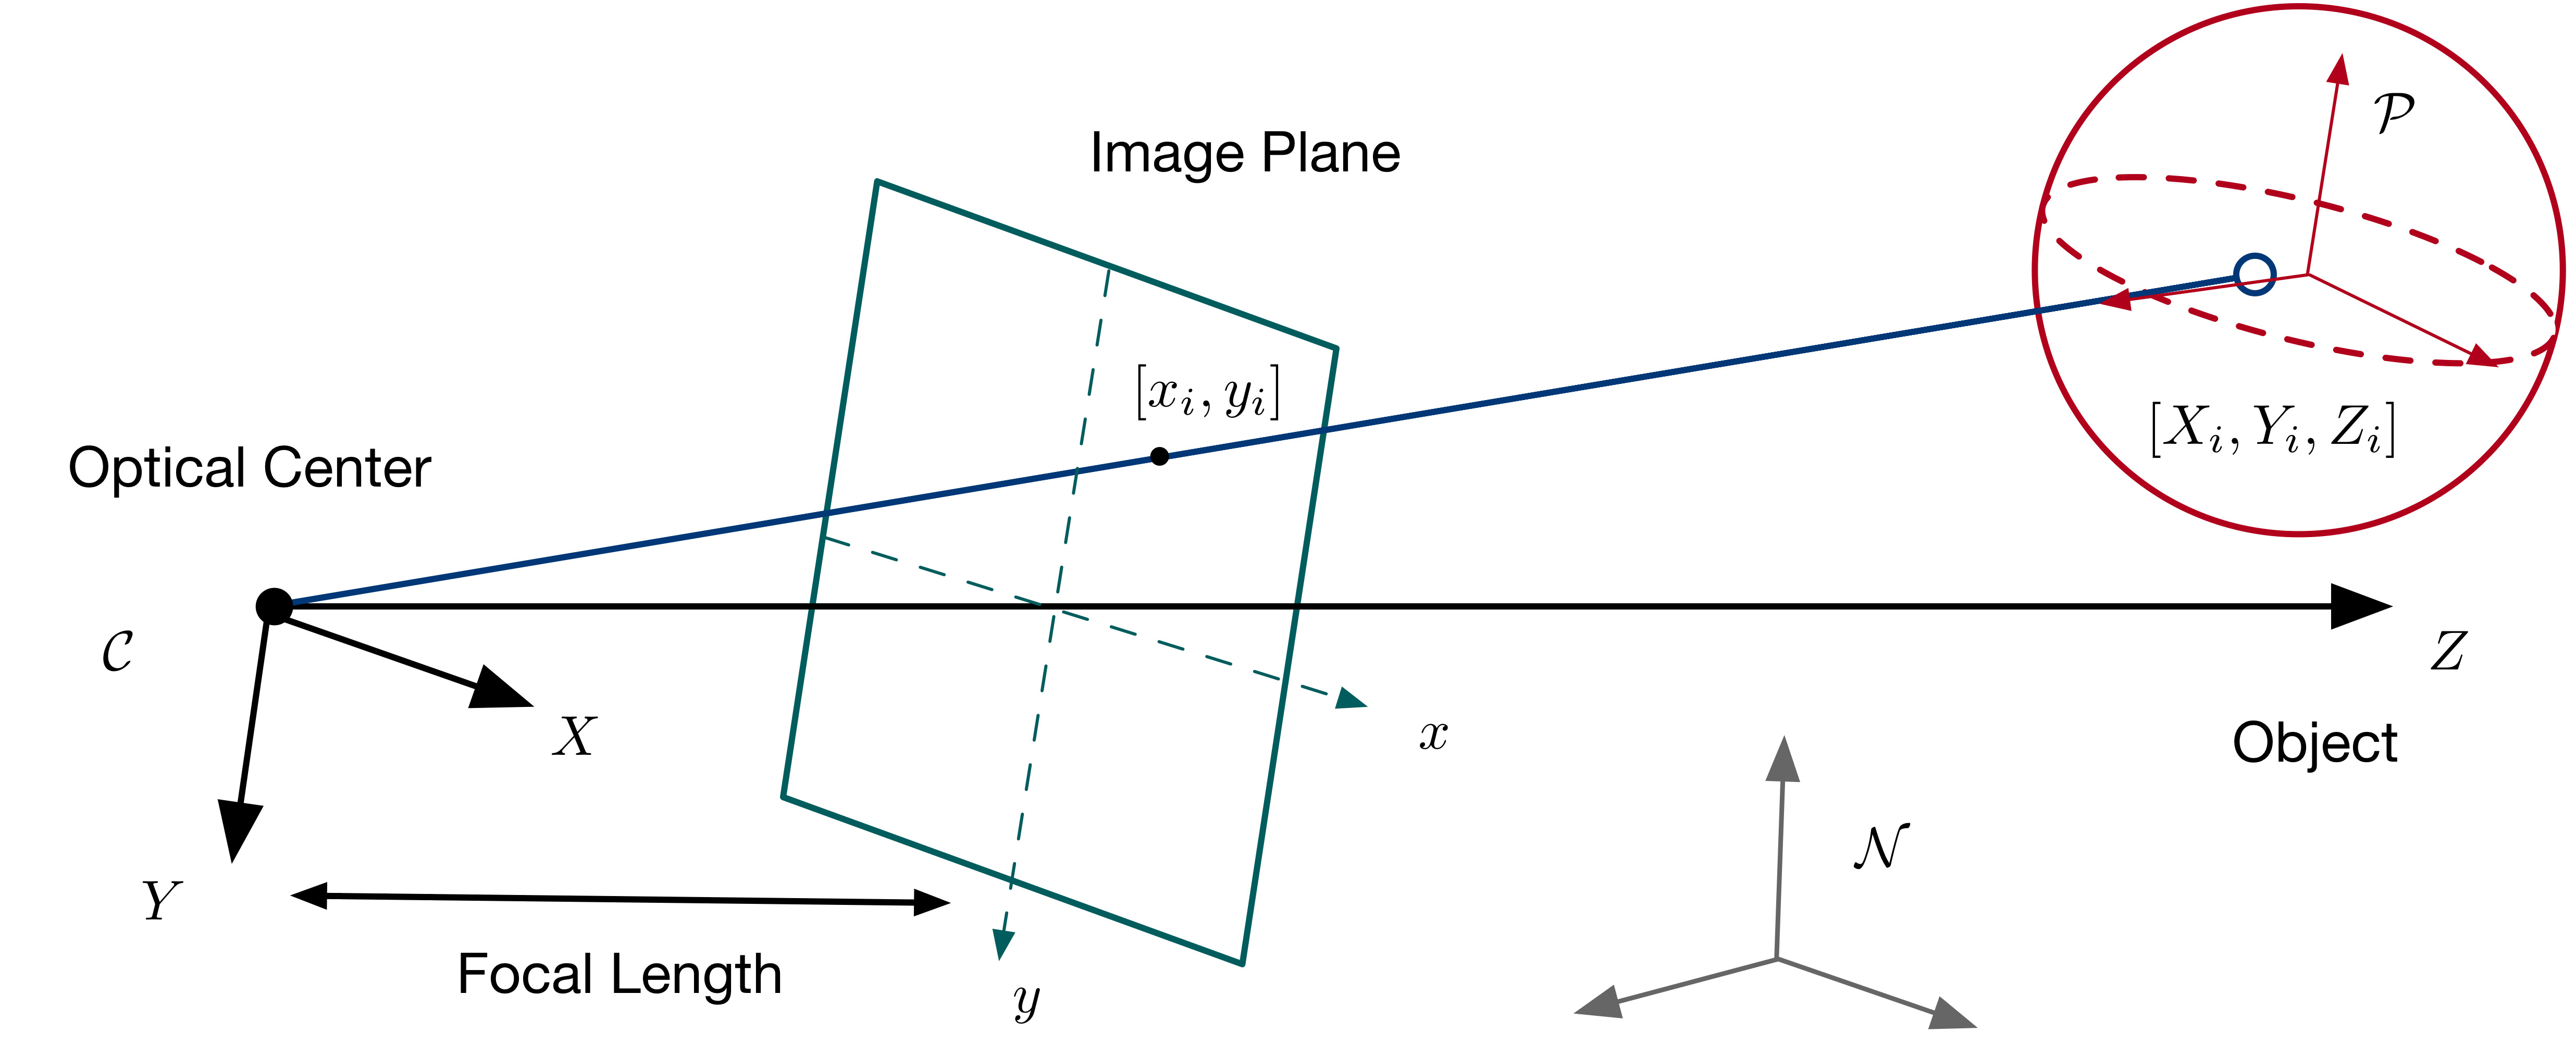
\includegraphics{Figures/CameraGeometry}
	}
	\caption{Camera Model}
	\label{fig:camera}
\end{figure}

\section{Model Description}

This converter module processes the output of a circle finding method to extract spacecraft inertial position. It does this by reading spacecraft attitude (coming from star tracker or other means), camera parameters, and the circle properties. 

Messages read:

\begin{itemize}
\item CameraConfigMsg: containing focal length, resolution, and sensor size. These values are needed for the following computations. Notably the camera frame relative to the body frame is used.
\item CirclesInMsg: Circle radius, center pixel and line, and uncertainty around these values in pixels. 
\item NavAttInMsg: Used for the spacecraft attitude. This allows to move from the body frame to the inertial frame.
\end{itemize}

